\documentclass[handout]{beamer}

\usepackage{Haust2017glærur}

\title{Stærðfræðimynstur í tölvunarfræði}
\subtitle{Vika 12, seinni fyrirlestur}

\begin{document}

\begin{frame}
\titlepage
\end{frame}


\section{Inngangur}

\begin{frame}{Í síðasta tíma}
    \begin{itemize}
        \item Lagnet
        \item Hnútalitun
    \end{itemize}
\end{frame}

\section{Stefnd rásalaus net}

\begin{frame}{Stefnd rásalaus net}
    \begin{columns}
        \column{0.5\textwidth}
        \begin{itemize}
            \item Stefnt rásalaust net (e. \emph{directed acyclic graphs}, DAG) er stefnt net án örvarása
            \item Klassískt dæmi: Skipulagning á forkröfum
            \item Hægt er að finna röðun (e. \emph{topological ordering}) á stefndu neti þá og því aðeins að það sé rásalaust
        \end{itemize}
        \column{0.5\textwidth}
        \begin{center}
            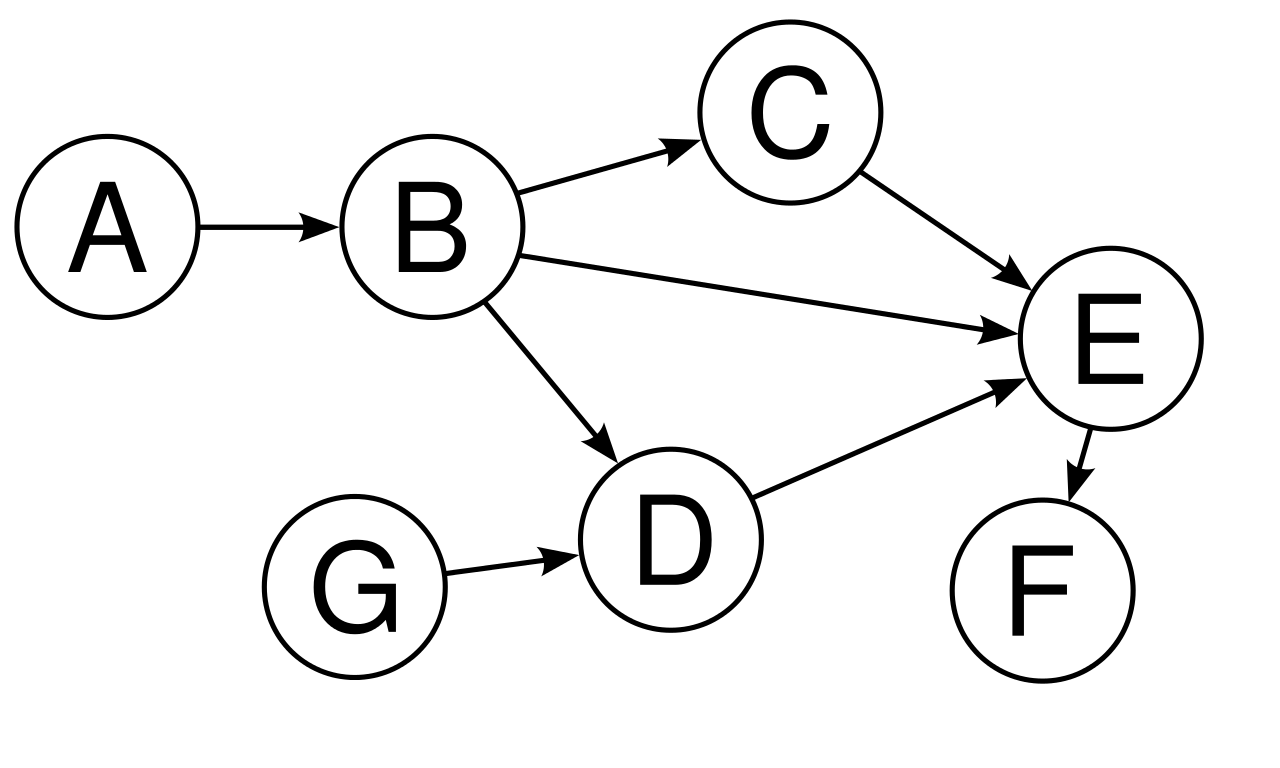
\includegraphics[width=\linewidth]{directed-acyclic-graph}
            
            Mynd: \href{https://commons.wikimedia.org/wiki/File:Directed_acyclic_graph.svg}{Wikipedia}
        \end{center}
    \end{columns}
\end{frame}

\begin{frame}{Dæmi}
    \vspace{\baselineskip}
    Getum notað stefnt rásalaust net til að hjálpa okkur að klæðast.
    
    \begin{center}
        \usetikzlibrary{arrows}
        \begin{tikzpicture}
            \tikzset{edge/.style = {->,> = latex'}}
            \node (a1) at (0, 4) {Nærbuxur};
            \node (b1) at (2, 1) {Sokkar};
            \node (c1) at (2, 3) {Buxur};
            \node (d1) at (3, 2) {Bolur};
            \node (e1) at (3, 4) {Peysa};
            \node (f1) at (0, 3) {Kápa};
            \node (g1) at (0, 1) {Skór};

            \draw[edge] (a1) to (c1);
            \draw[edge] (b1) to (g1);
            \draw[edge] (c1) to (f1);
            \draw[edge] (c1) to (g1);
            \draw[edge] (d1) to (e1);
            \draw[edge] (e1) to (f1);

            \node (a2) at (6, 0) {Nærbuxur};
            \node (b2) at (6, 0.8) {Sokkar};
            \node (c2) at (6, 1.6) {Buxur};
            \node (d2) at (6, 2.4) {Bolur};
            \node (e2) at (6, 3.2) {Peysa};
            \node (f2) at (6, 4.0) {Kápa};
            \node (g2) at (6, 4.8) {Skór};

            \draw[edge] (a2) to[bend left=70] (c2);
            \draw[edge] (b2) to[bend right=70] (g2);
            \draw[edge] (c2) to[bend right=70] (f2);
            \draw[edge] (c2) to[bend left=70] (g2);
            \draw[edge] (d2) to (e2);
            \draw[edge] (e2) to (f2);
        \end{tikzpicture}
    \end{center}
\end{frame}

\begin{frame}{Git}
    Í dag er Git vinsælasta kerfið til að sjá um útgáfustjórnun (e. \emph{version control}) í hugbúnaði. 
    Git byggist á stefndum rásalausum netum þar sem hver hnútur táknar ástand forritstexta.

    \begin{center}
        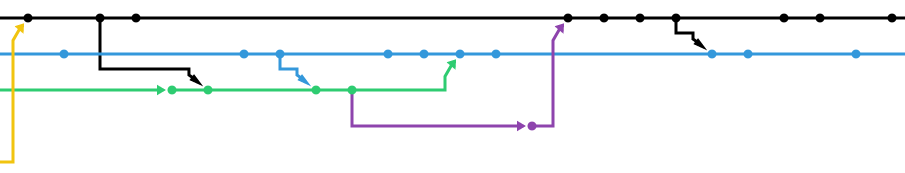
\includegraphics[width=\textwidth]{git-dag}
    \end{center}
\end{frame}

\begin{frame}[fragile]{Git dæmi}
\begin{minted}{bash}
$ git init # Tóm git-lind búin til
$ echo "prufutexti" > skra.txt
$ cat skra.txt 
prufutexti
$ git add skra.txt && git commit -m "Nýr hnútur búinn til"
$ echo "Nýr texti" > skra.txt # Skránni breytt
$ cat skra.txt
Nýr texti
$ git add skra.txt && git commit -m "Annar hnútur"
$ git checkout HEAD~1 # Bakkað um einn hnút
$ cat skra.txt # Skráin er nú í upphaflegu ástandi
prufutexti
\end{minted}
\end{frame}

\section{Tré}

\begin{frame}{Tré}
Skoðum nú sérstaka gerð neta, sem kölluð er \emph{tré}. Tvær jafngildar skilgreiningar eru:

\begin{tcolorbox}[title=Tré]
Tré (e. \emph{tree}) er samanhangandi óstefnt net án einfaldra rása.
\end{tcolorbox}

\begin{tcolorbox}[title=Tré]
Óstefnt net er tré sé til nákvæmlega einn einfaldur vegur á milli hverra tveggja hnúta í netinu.
\end{tcolorbox}

\end{frame}

\begin{frame}{Dæmi}
Netin $G_1$ og $G_2$ eru tré, en $G_3$ og $G_4$ ekki.
\begin{center}
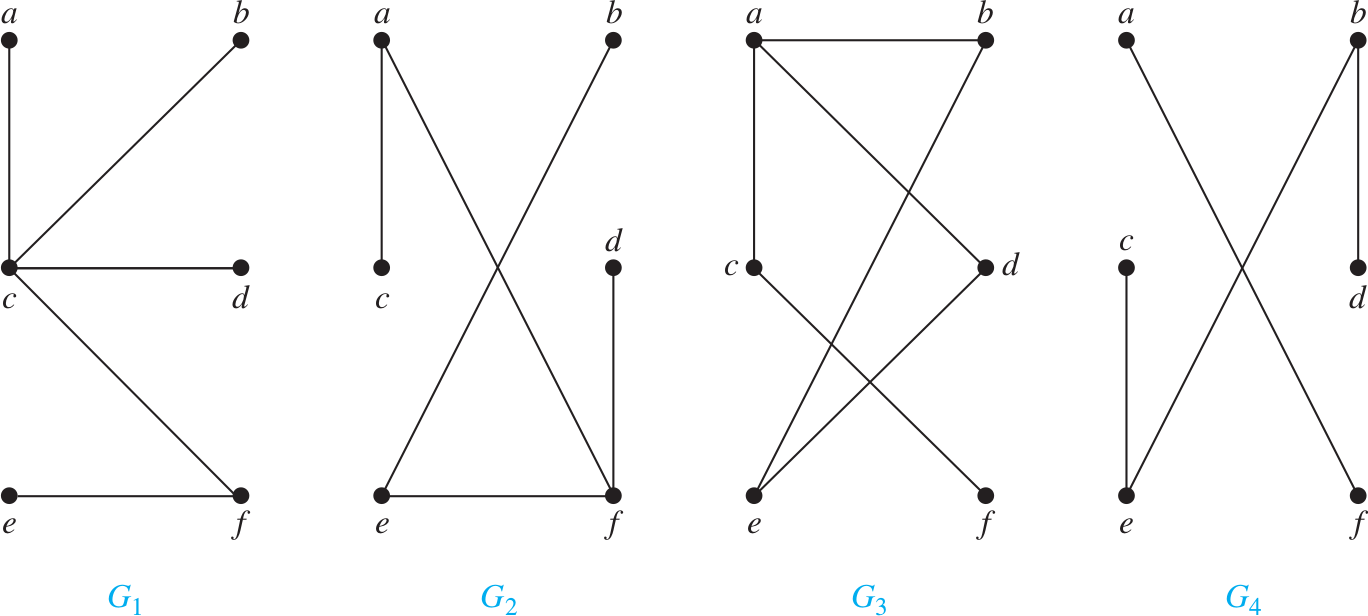
\includegraphics[width=\textwidth]{tree-not-trees}
\end{center}
\end{frame}

\begin{frame}{Skógur}
\begin{tcolorbox}[title=Skógur]
Net sem inniheldur engar einfaldar rásir er skógur (e. \emph{forest}). Skógur þarf ekki að vera samanhangandi. Hver samhengisþáttur skógar er tré.
\end{tcolorbox}
Skógur með þremur samhengisþáttum:
\begin{center}
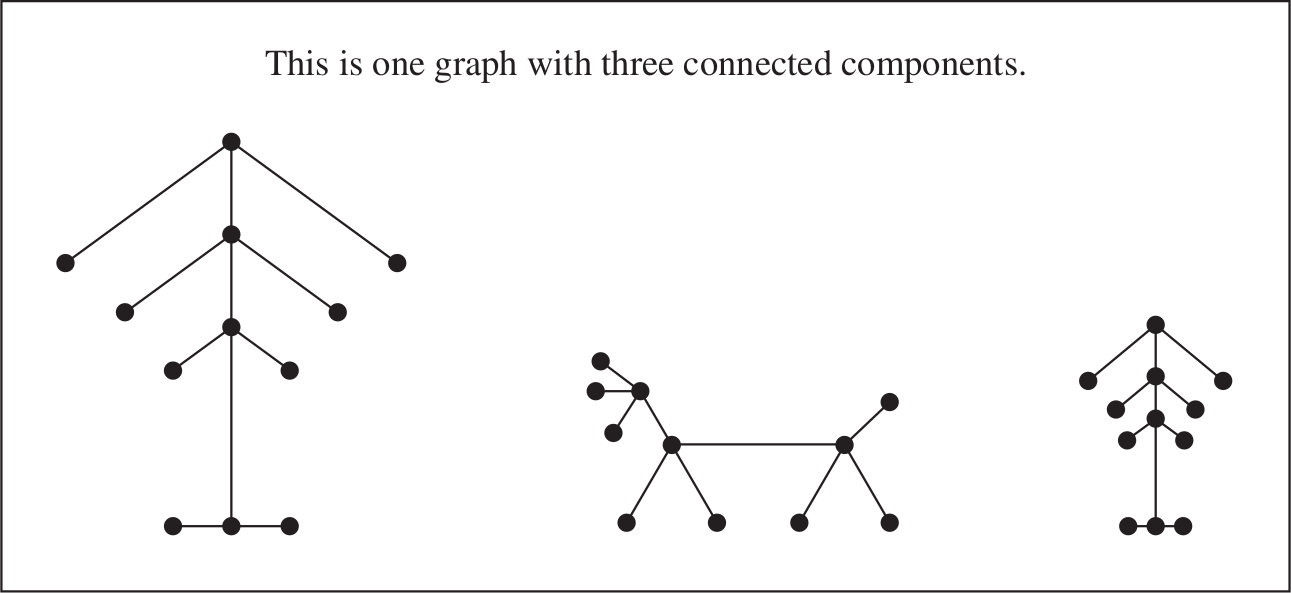
\includegraphics[width=0.8\textwidth]{tree-forest}
\end{center}
\end{frame}

\begin{frame}{Rótartré}
\begin{tcolorbox}[title=Rótartré]
Rótfast tré eða rótartré (e. \emph{rooted tree}) er tré þar sem einn hnútur hefur verið skilgreindur sem rót (e. \emph{root}). Hafi rótartré stefnu er stefna hvers leggs í átt frá rótinni.
\end{tcolorbox}
Tré $T$ og aðskilin rótartré mynduð út frá því:
\begin{center}
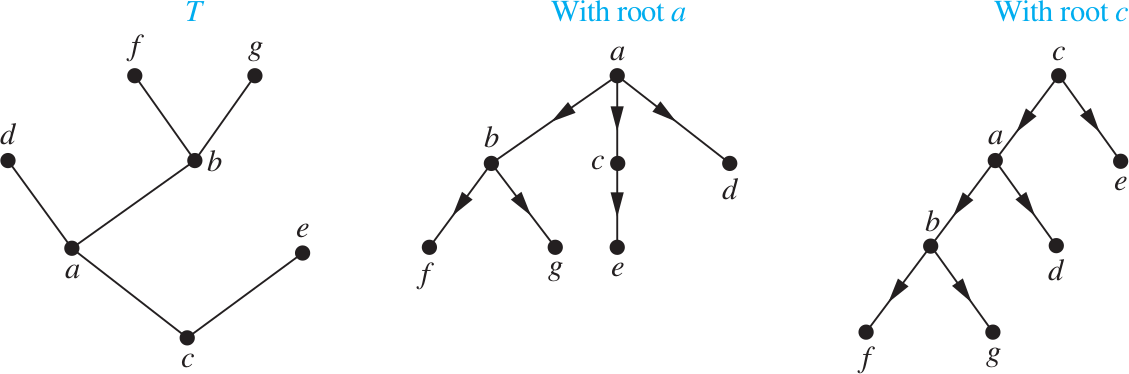
\includegraphics[width=0.8\textwidth]{tree-rooted}
\end{center}
\end{frame}

\begin{frame}{Dæmi}
\href{https://upload.wikimedia.org/wikipedia/commons/1/1b/Linux_Distribution_Timeline.svg}{``Ættarskógur'' Linux}
\end{frame}

\begin{frame}{Skráarkerfi}
\begin{center}
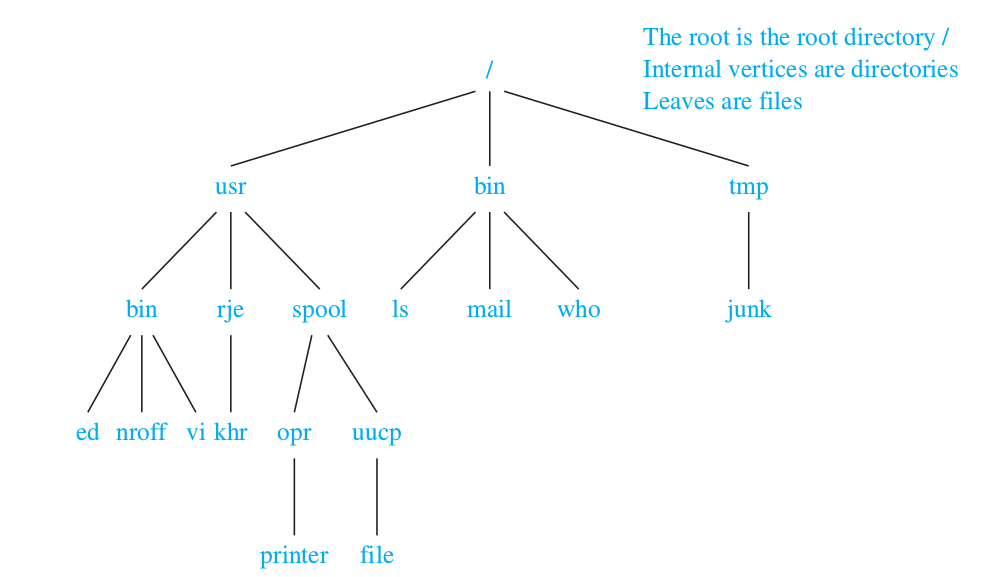
\includegraphics[width=0.7\textwidth]{tree-file-system}
\end{center}
\end{frame}

\begin{frame}{Hugtök}
\begin{itemize}
 \item Fjölmörg hugtök eru skilgreind fyrir tré og rótartré
 \item Hugtök nefnd eftir ættartengslum:
 \begin{itemize}
  \item Foreldri (e. \emph{parent}) hnúts $v$ í rótartré $T$ er eini hnúturinn $u$ í $T$ svo að $(u,v)$ sé örvaleggur
  \item Börn (e. \emph{children}) hnúts $v$ eru þeir hnútar $T$ sem hafa $v$ sem foreldri
  \item Systkin (e. \emph{siblings}) eru hnútar sem eiga sama foreldri
  \item Áar (e. \emph{ancestors}) hnúts $v$ eru þeir hnútar sem eru hluti af vegi frá rót til $v$, að $v$ sjálfum undanskildum
  \item Afkomendur (e. \emph{descendents}) hnúts $v$ eru þeir hnútar sem hafa $v$ sem áa
 \end{itemize}
\end{itemize}
\end{frame}

\begin{frame}{Hugtök}
\begin{itemize}
 \item Fleiri hugtök:
 \begin{itemize}
  \item Lauf (e. \emph{leaf}) er hnútur í tré af stigi 1
  \begin{itemize}
   \item Í rótartré má skilgreina lauf sem hnút sem á engin börn
  \end{itemize}
  \item Innri hnútur (e. \emph{internal vertex}) er hnútur í tré sem ekki er lauf
  \item Hluttré (e. \emph{subtree}) rótartrésins $T$ er rótartré $T'$ sem myndað er með hnút $a$ úr $T$ ásamt öllum afkomendum $a$ og öllum aðlægum leggjum afkomendanna
  \item Hæð (e. \emph{height}) rótartrés er fjöldi leggja í veg frá rót til laufs
  \begin{itemize}
   \item Rótin er í hæð 0
  \end{itemize}
 \end{itemize}
\end{itemize}
\end{frame}


\begin{frame}{$m$-undartré}
Rótartré sem hafa þann eiginleika að hnútarnir hafa hámarksfjölda barna koma víða við
\begin{tcolorbox}[title=$m$-undartré]
Rótartré er $m$-undartré (e. \emph{$m$-ary tree}) hafi hver innri hnútur þess að hámarki $m$ börn. Rótartré er kallað fullskipað $m$-undartré (e. \emph{full $m$-ary tree}) hafi hver innri hnútur þess nákvæmlega $m$ börn.
\end{tcolorbox}

$m$-undartré með $m = 2$ er kallað tvíundartré (e. \emph{binary tree}).
\end{frame}

\begin{frame}{Dæmi}
\begin{center}
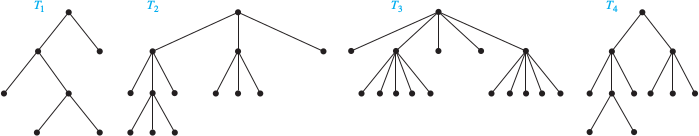
\includegraphics[width=\textwidth]{tree-full}
\end{center}
Hver þessara trjáa eru fullskipuð $m$-undartré fyrir eitthvert gildi á $m$?
\end{frame}

\begin{frame}{Röðuð rótartré}
\begin{itemize}
 \item Við getum skilgreint röðun á börn hvers hnúts í rótartré
 \begin{itemize}
  \item Getur verið mikilvægt í reikniritum
 \end{itemize}
 \item Í röðuðu tvíundartré getum við talað um ``vinstra barn'' og ``hægra barn'' einhvers hnúts
 \item Sömuleiðis getum við skilgreint ``vinstra hluttré'' og ``hægra hluttré'' fyrir einhvern hnút í rótartré
\end{itemize}
\end{frame}

\subsection{Eiginleikar trjáa}

\begin{frame}{Eiginleikar trjáa}
Við getum sett fram ýmsar staðhæfingar um samband hnúta- og leggjafjölda trjáa. Tré eru afmarkaðra fyrirbrigði en net, svo við getum sett fram sterkari staðhæfingar.

\begin{tcolorbox}
Tré með $n$ hnútum hefur $n-1$ leggi.
\end{tcolorbox}

\begin{tcolorbox}
Fullskipað $m$-undartré með $i$ innri hnúta hefur $n = mi +1$ hnúta.
\end{tcolorbox}
\end{frame}

\begin{frame}{Jafnvægi}
Oft er æskilegt að rótartré séu ``í jafnvægi''. Rótartré er í jafnvægi sé hámarksmismunur á lengd allra vega frá rót að laufi 1.

\vspace{0.5cm}
Sum eftirfarandi trjáa eru í jafnvægi:
\begin{center}
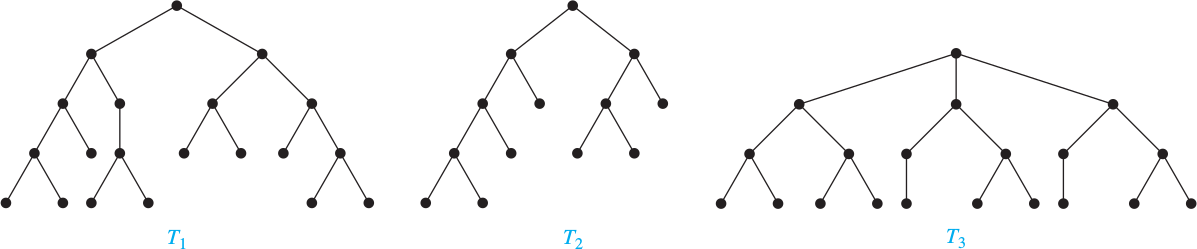
\includegraphics[width=\textwidth]{tree-balanced}
\end{center}
\pause
Það eru $T_1$ og $T_3$.
\end{frame}

\begin{frame}{Fleiri eiginleikar trjáa}
Vitum við hæð trés getum við sett skorður á laufafjöldann.
\begin{tcolorbox}
$m$-undartré af hæð $h$ hefur að hámarki $l = m^h$ lauf.
\end{tcolorbox}

\begin{tcolorbox}
$m$-undartré af hæð $h$ með $l$ lauf hefur $h \geq \lceil \log_m l \rceil$. Sé $m$-undartréð fullskipað og í jafnvægi, þá er $h = \lceil \log_m l\rceil$.
\end{tcolorbox}
\end{frame}

\section{Hagnýtingar á trjám}

\begin{frame}{Tvíleitartré}
\begin{itemize}
 \item Ein algengasta gerð verkefna sem kemur upp í tölvunarfræði er leitarverkefni
 \item Tvíleitartré (e. \emph{binary search tree}) eru mjög gagnleg þegar setja þarf upp ýmis leitarverkefni
 \item Tvíleitartré er raðað tvíundartré
 \begin{itemize}
  \item Hver hnútur er merktur með ``lykli'' (e. \emph{key})
  \begin{itemize}
   \item Við þurfum að geta borið tvo lykla saman til að athuga hvor þeirra sé stærri
  \end{itemize}
  \item Tréð er þannig upp byggt að allir lyklar í vinstra undirtré hnúts $v$ eru minni en lykill $v$, allir lyklar í hægra undirtré hnúts $v$ eru ekki minni en lykill $v$
 \end{itemize}
 \item Mjög auðvelt er að útfæra helmingunarleit sem virkar á tvíleitartré
\end{itemize}
\end{frame}

\begin{frame}{Raðað inn í tvíleitartré}
Hér eru lyklar strengir, raðað í stafrófsröð:
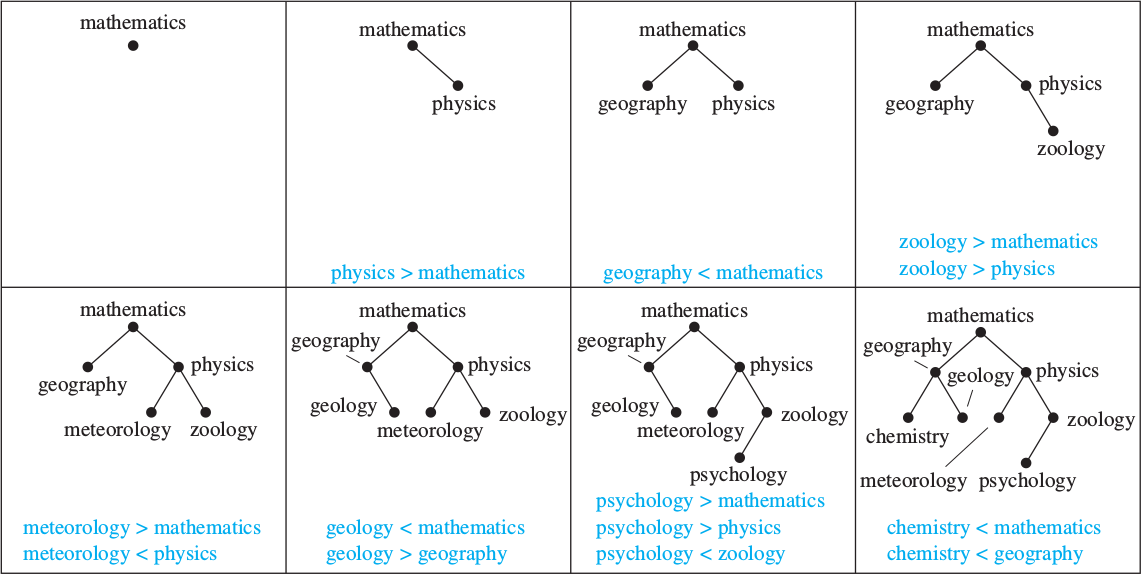
\includegraphics[width=\textwidth]{tree-subjects-search}
\end{frame}

\begin{frame}{Ákvarðanatré}
\begin{itemize}
 \item Við getum látið rótartré tákna mögulegar ákvarðanir í forriti
 \begin{itemize}
  \item Látum þá hvern hnút tákna ástand
  \item Börn hvers hnúts tákna mögulegar ákvarðanir sem hægt er að taka í því ástandi
 \end{itemize}
 \item Getum myndað einfalda ``gervigreind'' með þessum hætti
 \item Mjög svipað hugtak - leikjatré
\end{itemize}
\end{frame}

\begin{frame}{Leikjatré myllu}
\begin{center}
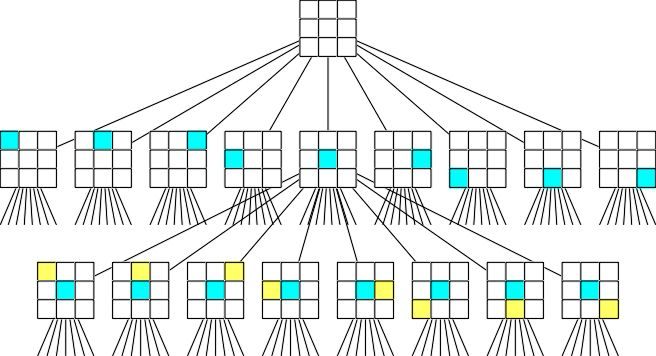
\includegraphics[width=\textwidth]{tic-tac-toe}
\end{center}
\end{frame}

\section{Fjöldi samanburða í röðun}

\begin{frame}{Fjöldi samanburða}
\begin{center}
Athugum ákvarðanatré fyrir röðun á þremur stökum $a, b$ og $c$:

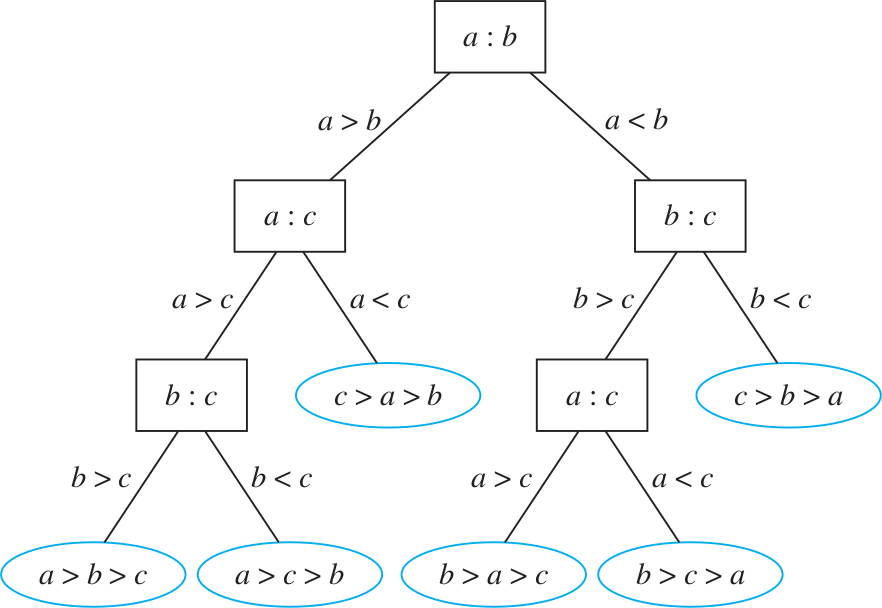
\includegraphics[width=0.7\textwidth]{tree-comparison-decision}
\end{center}
\end{frame}

\begin{frame}{Fjöldi samanburða}
    \begin{itemize}
        \item Rifjum upp: Fjöldi umraðana á $n$ stökum er $n!$ \pause
        \begin{itemize}
            \item Þetta er fjöldi laufa í ákvarðanatré röðunar
        \end{itemize}
            \item Munum enn: Um $m$-undartré af hæð $h$ með $l$ lauf gildir $h \geq \lceil \log_m l\rceil$ \pause
        \begin{itemize}
            \item Afleiðing: Við þurfum $\lceil \log_m n! \rceil$ einfalda samanburði til að raða $n$ stökum \pause
        \end{itemize}
            \item Rifjum upp: $\log n!$ er $\Theta(n \log n)$ \pause
        \begin{itemize}
            \item Afleiðing: Fjöldi samanburða sem röðunarreiknirit sem ber saman öll stökin þarf er $\Omega(n\log n)$
            \item Merge sort nær þessu!
        \end{itemize}
    \end{itemize}
\end{frame}

\section{Trjáflakk}

\begin{frame}{Trjáflakk}
\begin{itemize}
 \item Tré eru skipuleg fyrirbrigði, þess vegna er auðvelt að kanna þau skipulega
 \begin{itemize}
  \item Mun auðveldara er að fara skipulega í gegnum tré en almennt net!
 \end{itemize}
 \item Skoðum sérstaklega leiðir til að kanna röðuð rótartré
 \item ``Skrifum út'' lista af gildum hnúta
 \begin{itemize}
  \item Förum alltaf sama hring í gegnum tréð, en listinn verður mismunandi eftir röð aðgerða
 \end{itemize}
\end{itemize}
\end{frame}

\begin{frame}[fragile]{Fyrirröð}
    Getum skilgreint trjáflakk í fyrirröð (e. \emph{preorder traversal}).

    \begin{center}
        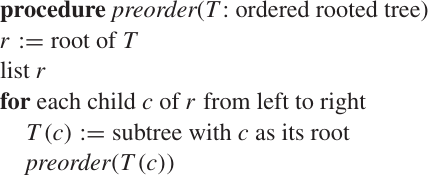
\includegraphics[width=0.7\textwidth]{preorder-algorithm}
    \end{center}
\end{frame}

\begin{frame}[fragile]{Miðröð}
    Getum skilgreint trjáflakk í miðröð (e. \emph{inorder}).

    \begin{center}
        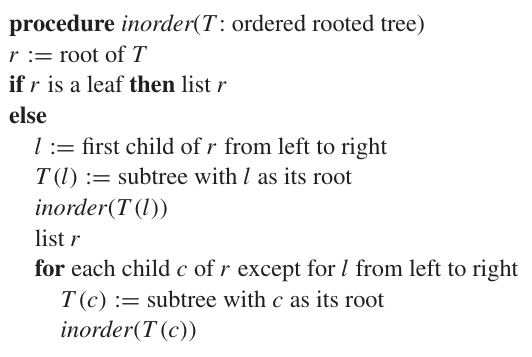
\includegraphics[width=0.5\textwidth]{inorder-algorithm}
    \end{center}

Miðröð kemur mjög oft fyrir, því að hún skrifar út tvíleitartré í réttri röð.
\end{frame}

\begin{frame}[fragile]{Eftirröð}
Getum skilgreint trjáflakk í eftirröð (e. \emph{postorder}).

\begin{center}
    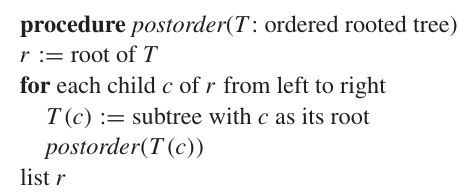
\includegraphics[width=0.7\textwidth]{postorder-algorithm}
\end{center}
\end{frame}

\begin{frame}{Samanburður}
\begin{columns}
\column{0.33\textwidth}
Fyrirröð
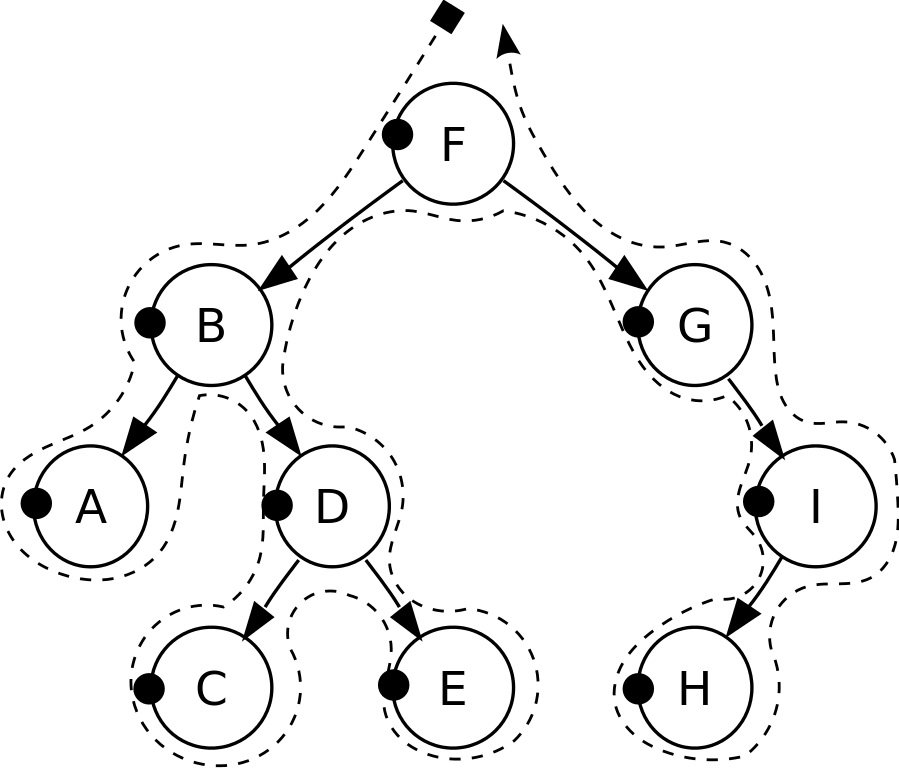
\includegraphics[width=\linewidth]{tree-preorder}
\[F, B, A, D, C, E, G, I, H\]
\column{0.33\textwidth}
Miðröð
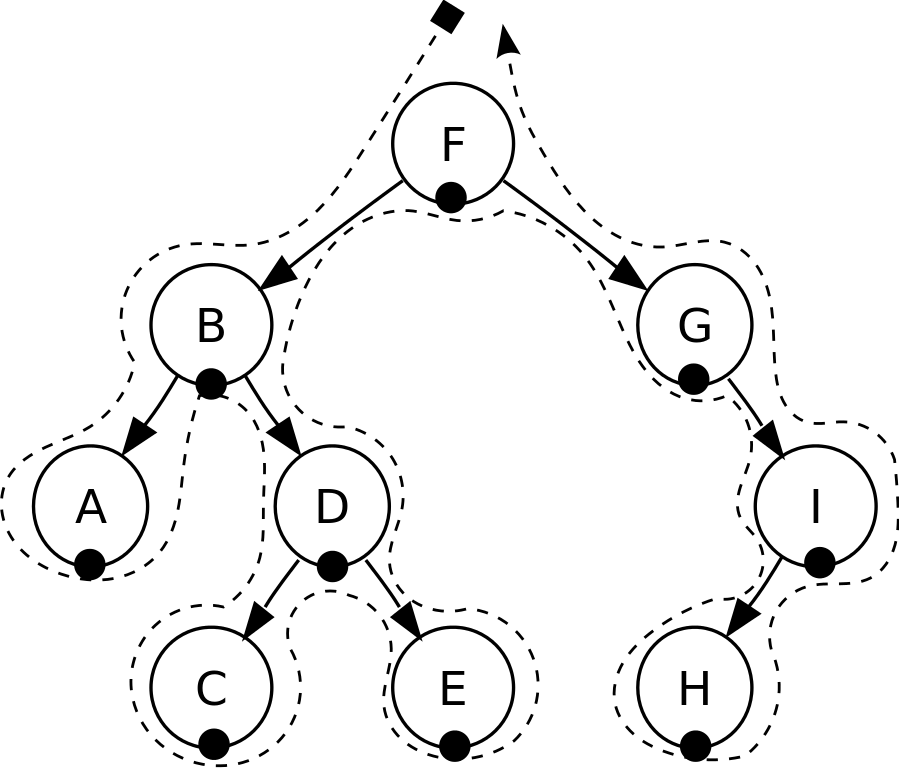
\includegraphics[width=\linewidth]{tree-inorder}
\[A, B, C, D, E, F, G, H, I\]
\column{0.33\textwidth}
Eftirröð
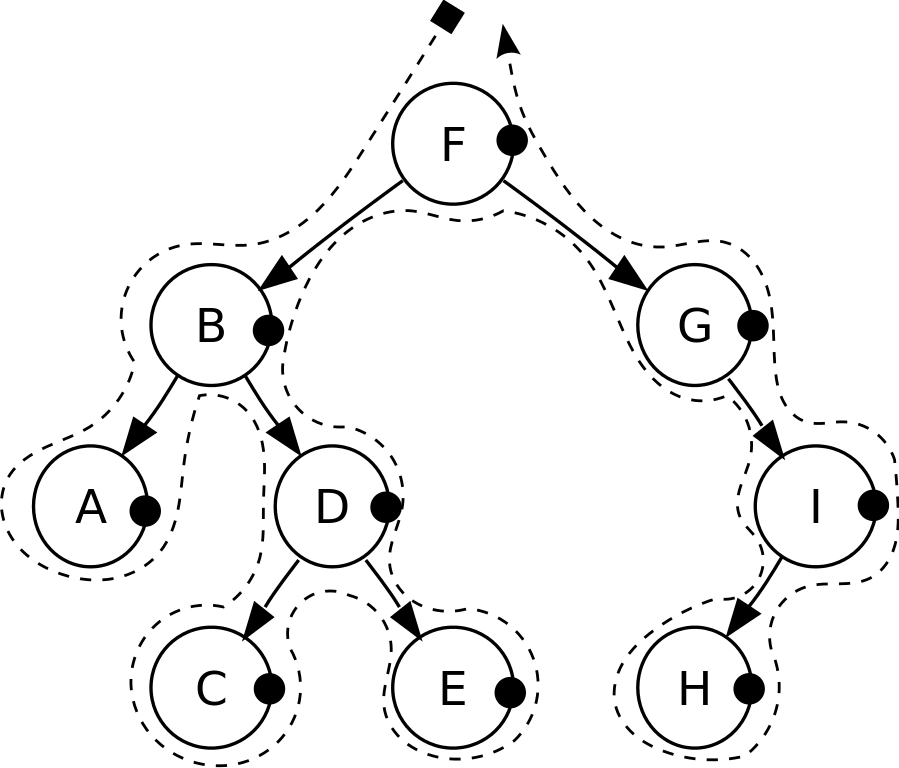
\includegraphics[width=\linewidth]{tree-postorder}
\[A, C, E, D, B, H, I, G, F\]
\end{columns}

\end{frame}



\begin{frame}{Næst}
Spanntré (11.4 og 11.5).
\end{frame}


\end{document}
